\documentclass[14pt]{extbook}
\usepackage{multicol, enumerate, enumitem, hyperref, color, soul, setspace, parskip, fancyhdr} %General Packages
\usepackage{amssymb, amsthm, amsmath, bbm, latexsym, units, mathtools} %Math Packages
\everymath{\displaystyle} %All math in Display Style
% Packages with additional options
\usepackage[headsep=0.5cm,headheight=12pt, left=1 in,right= 1 in,top= 1 in,bottom= 1 in]{geometry}
\usepackage[usenames,dvipsnames]{xcolor}
\usepackage{dashrule}  % Package to use the command below to create lines between items
\newcommand{\litem}[1]{\item#1\hspace*{-1cm}\rule{\textwidth}{0.4pt}}
\pagestyle{fancy}
\lhead{Module6}
\chead{}
\rhead{Version C}
\lfoot{9356-6875}
\cfoot{}
\rfoot{testing}
\begin{document}

\begin{enumerate}
\litem{
Describe the end behavior of the polynomial below.\[ f(x) = -3(x - 8)^{5}(x + 8)^{10}(x - 6)^{3}(x + 6)^{5} \]\begin{enumerate}[label=\Alph*.]
\begin{multicols}{2}\item 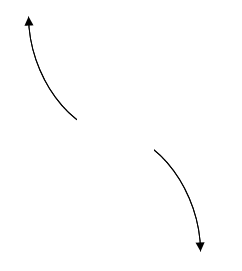
\includegraphics[width = 0.3\textwidth]{../Figures/polyEndBehaviorAC.png}\item 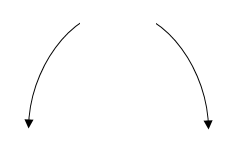
\includegraphics[width = 0.3\textwidth]{../Figures/polyEndBehaviorBC.png}\item 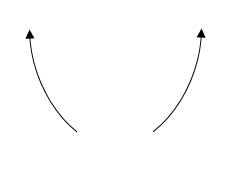
\includegraphics[width = 0.3\textwidth]{../Figures/polyEndBehaviorCC.png}\item 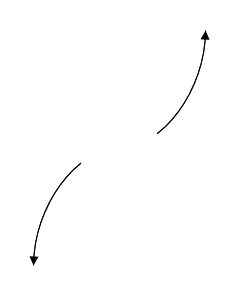
\includegraphics[width = 0.3\textwidth]{../Figures/polyEndBehaviorDC.png}\end{multicols}\item None of the above.
\end{enumerate} }
\litem{
Which of the following equations \textit{could} be of the graph presented below?
\begin{center}
    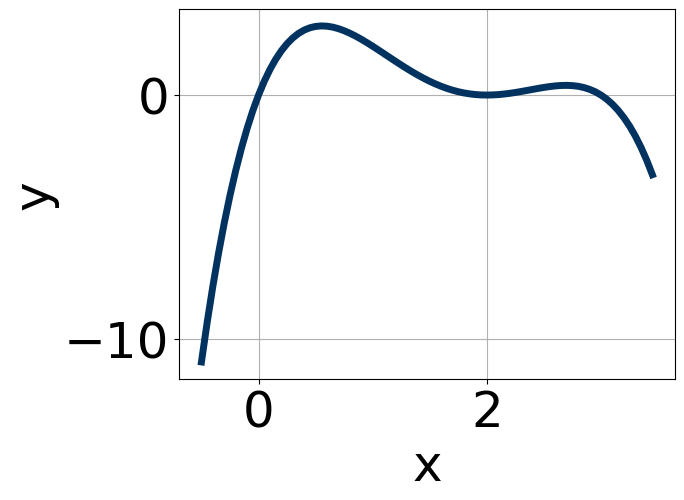
\includegraphics[width=0.5\textwidth]{../Figures/polyGraphToFunctionC.png}
\end{center}
\begin{enumerate}[label=\Alph*.]
\item \( 20x^{9} (x - 2)^{6} (x - 3)^{6} \)
\item \( -3x^{6} (x - 2)^{11} (x - 3)^{11} \)
\item \( 14x^{9} (x - 2)^{6} (x - 3)^{7} \)
\item \( -19x^{6} (x - 2)^{10} (x - 3)^{9} \)
\item \( -13x^{5} (x - 2)^{8} (x - 3)^{9} \)

\end{enumerate} }
\litem{
Construct the lowest-degree polynomial given the zeros below. Then, choose the intervals that contain the coefficients of the polynomial in the form $ax^3+bx^2+cx+d$.\[ 7, \frac{-4}{5}, \text{ and } \frac{-3}{2} \]\begin{enumerate}[label=\Alph*.]
\item \( a \in [8, 12], b \in [88, 101], c \in [170, 175], \text{ and } d \in [81, 90] \)
\item \( a \in [8, 12], b \in [-49, -45], c \in [-149, -146], \text{ and } d \in [-84, -79] \)
\item \( a \in [8, 12], b \in [44, 52], c \in [-149, -146], \text{ and } d \in [81, 90] \)
\item \( a \in [8, 12], b \in [76, 78], c \in [36, 43], \text{ and } d \in [-84, -79] \)
\item \( a \in [8, 12], b \in [-49, -45], c \in [-149, -146], \text{ and } d \in [81, 90] \)

\end{enumerate} }
\litem{
Construct the lowest-degree polynomial given the zeros below. Then, choose the intervals that contain the coefficients of the polynomial in the form $x^3+bx^2+cx+d$.\[ 4 - 2 i \text{ and } 1 \]\begin{enumerate}[label=\Alph*.]
\item \( b \in [-5, 6], c \in [-5, -1], \text{ and } d \in [-1, 8] \)
\item \( b \in [7, 10], c \in [25, 33], \text{ and } d \in [17, 23] \)
\item \( b \in [-5, 6], c \in [-4, 3], \text{ and } d \in [-4, -1] \)
\item \( b \in [-12, -4], c \in [25, 33], \text{ and } d \in [-21, -15] \)
\item \( \text{None of the above.} \)

\end{enumerate} }
\litem{
Construct the lowest-degree polynomial given the zeros below. Then, choose the intervals that contain the coefficients of the polynomial in the form $ax^3+bx^2+cx+d$.\[ \frac{3}{5}, \frac{7}{2}, \text{ and } 3 \]\begin{enumerate}[label=\Alph*.]
\item \( a \in [9, 13], b \in [-61, -58], c \in [60, 69], \text{ and } d \in [58, 67] \)
\item \( a \in [9, 13], b \in [65, 75], c \in [143, 149], \text{ and } d \in [58, 67] \)
\item \( a \in [9, 13], b \in [11, 13], c \in [-103, -100], \text{ and } d \in [-72, -62] \)
\item \( a \in [9, 13], b \in [-72, -62], c \in [143, 149], \text{ and } d \in [58, 67] \)
\item \( a \in [9, 13], b \in [-72, -62], c \in [143, 149], \text{ and } d \in [-72, -62] \)

\end{enumerate} }
\litem{
Construct the lowest-degree polynomial given the zeros below. Then, choose the intervals that contain the coefficients of the polynomial in the form $x^3+bx^2+cx+d$.\[ -3 - 5 i \text{ and } -2 \]\begin{enumerate}[label=\Alph*.]
\item \( b \in [-6, 3], c \in [4.7, 6.1], \text{ and } d \in [5.4, 9.1] \)
\item \( b \in [-6, 3], c \in [5.7, 8.3], \text{ and } d \in [8.4, 11.7] \)
\item \( b \in [-8, -2], c \in [44, 46.1], \text{ and } d \in [-69.7, -66.9] \)
\item \( b \in [7, 15], c \in [44, 46.1], \text{ and } d \in [63.1, 71.7] \)
\item \( \text{None of the above.} \)

\end{enumerate} }
\litem{
Describe the end behavior of the polynomial below.\[ f(x) = 4(x + 2)^{4}(x - 2)^{9}(x + 9)^{3}(x - 9)^{4} \]\begin{enumerate}[label=\Alph*.]
\begin{multicols}{2}\item 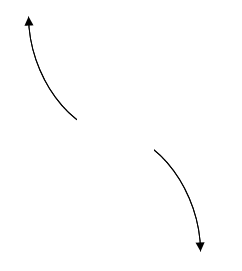
\includegraphics[width = 0.3\textwidth]{../Figures/polyEndBehaviorCopyAC.png}\item 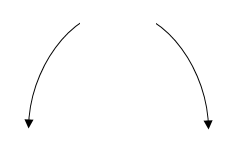
\includegraphics[width = 0.3\textwidth]{../Figures/polyEndBehaviorCopyBC.png}\item 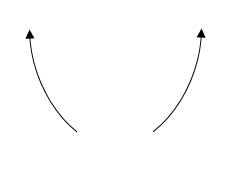
\includegraphics[width = 0.3\textwidth]{../Figures/polyEndBehaviorCopyCC.png}\item 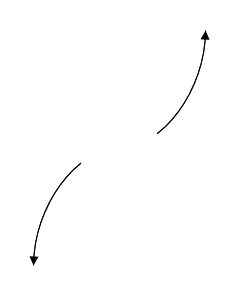
\includegraphics[width = 0.3\textwidth]{../Figures/polyEndBehaviorCopyDC.png}\end{multicols}\item None of the above.
\end{enumerate} }
\litem{
Describe the zero behavior of the zero $x = -2$ of the polynomial below.\[ f(x) = -8(x - 6)^{11}(x + 6)^{9}(x - 2)^{5}(x + 2)^{4} \]\begin{enumerate}[label=\Alph*.]
\begin{multicols}{2}\item 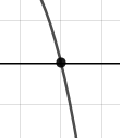
\includegraphics[width = 0.3\textwidth]{../Figures/polyZeroBehaviorAC.png}\item 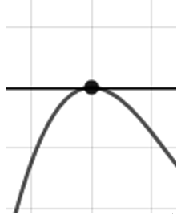
\includegraphics[width = 0.3\textwidth]{../Figures/polyZeroBehaviorBC.png}\item 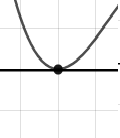
\includegraphics[width = 0.3\textwidth]{../Figures/polyZeroBehaviorCC.png}\item 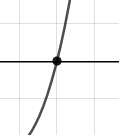
\includegraphics[width = 0.3\textwidth]{../Figures/polyZeroBehaviorDC.png}\end{multicols}\item None of the above.
\end{enumerate} }
\litem{
Describe the zero behavior of the zero $x = -2$ of the polynomial below.\[ f(x) = -4(x + 5)^{9}(x - 5)^{5}(x + 2)^{10}(x - 2)^{9} \]\begin{enumerate}[label=\Alph*.]
\begin{multicols}{2}\item 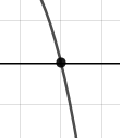
\includegraphics[width = 0.3\textwidth]{../Figures/polyZeroBehaviorCopyAC.png}\item 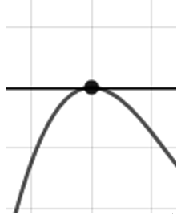
\includegraphics[width = 0.3\textwidth]{../Figures/polyZeroBehaviorCopyBC.png}\item 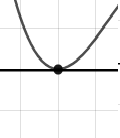
\includegraphics[width = 0.3\textwidth]{../Figures/polyZeroBehaviorCopyCC.png}\item 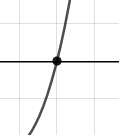
\includegraphics[width = 0.3\textwidth]{../Figures/polyZeroBehaviorCopyDC.png}\end{multicols}\item None of the above.
\end{enumerate} }
\litem{
Which of the following equations \textit{could} be of the graph presented below?
\begin{center}
    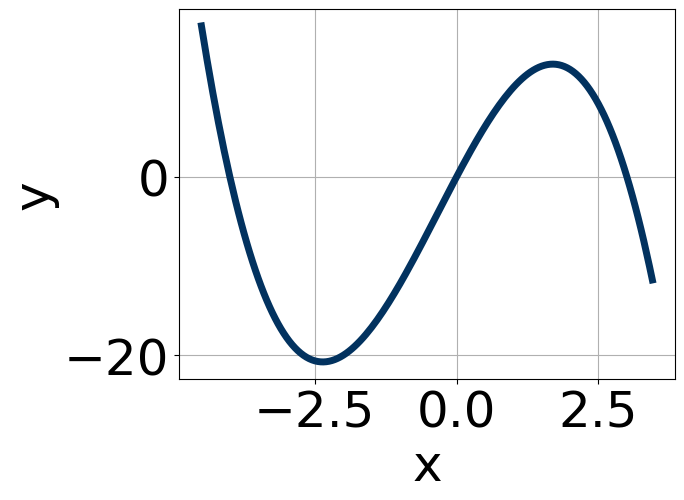
\includegraphics[width=0.5\textwidth]{../Figures/polyGraphToFunctionCopyC.png}
\end{center}
\begin{enumerate}[label=\Alph*.]
\item \( -18x^{10} (x + 3)^{6} (x + 4)^{8} \)
\item \( 7x^{5} (x + 3)^{6} (x + 4)^{6} \)
\item \( -14x^{8} (x + 3)^{10} (x + 4)^{9} \)
\item \( 2x^{5} (x + 3)^{10} (x + 4)^{7} \)
\item \( 19x^{6} (x + 3)^{8} (x + 4)^{11} \)

\end{enumerate} }
\end{enumerate}

\end{document}